\documentclass[]{article}
\usepackage{lmodern}
\usepackage{amssymb,amsmath}
\usepackage{ifxetex,ifluatex}
\usepackage{fixltx2e} % provides \textsubscript
\ifnum 0\ifxetex 1\fi\ifluatex 1\fi=0 % if pdftex
  \usepackage[T1]{fontenc}
  \usepackage[utf8]{inputenc}
\else % if luatex or xelatex
  \ifxetex
    \usepackage{mathspec}
  \else
    \usepackage{fontspec}
  \fi
  \defaultfontfeatures{Ligatures=TeX,Scale=MatchLowercase}
\fi
% use upquote if available, for straight quotes in verbatim environments
\IfFileExists{upquote.sty}{\usepackage{upquote}}{}
% use microtype if available
\IfFileExists{microtype.sty}{%
\usepackage{microtype}
\UseMicrotypeSet[protrusion]{basicmath} % disable protrusion for tt fonts
}{}
\usepackage[margin=1in]{geometry}
\usepackage{hyperref}
\hypersetup{unicode=true,
            pdftitle={Homework 13},
            pdfauthor={Christophe Hunt},
            pdfborder={0 0 0},
            breaklinks=true}
\urlstyle{same}  % don't use monospace font for urls
\usepackage{graphicx,grffile}
\makeatletter
\def\maxwidth{\ifdim\Gin@nat@width>\linewidth\linewidth\else\Gin@nat@width\fi}
\def\maxheight{\ifdim\Gin@nat@height>\textheight\textheight\else\Gin@nat@height\fi}
\makeatother
% Scale images if necessary, so that they will not overflow the page
% margins by default, and it is still possible to overwrite the defaults
% using explicit options in \includegraphics[width, height, ...]{}
\setkeys{Gin}{width=\maxwidth,height=\maxheight,keepaspectratio}
\IfFileExists{parskip.sty}{%
\usepackage{parskip}
}{% else
\setlength{\parindent}{0pt}
\setlength{\parskip}{6pt plus 2pt minus 1pt}
}
\setlength{\emergencystretch}{3em}  % prevent overfull lines
\providecommand{\tightlist}{%
  \setlength{\itemsep}{0pt}\setlength{\parskip}{0pt}}
\setcounter{secnumdepth}{5}
% Redefines (sub)paragraphs to behave more like sections
\ifx\paragraph\undefined\else
\let\oldparagraph\paragraph
\renewcommand{\paragraph}[1]{\oldparagraph{#1}\mbox{}}
\fi
\ifx\subparagraph\undefined\else
\let\oldsubparagraph\subparagraph
\renewcommand{\subparagraph}[1]{\oldsubparagraph{#1}\mbox{}}
\fi

%%% Use protect on footnotes to avoid problems with footnotes in titles
\let\rmarkdownfootnote\footnote%
\def\footnote{\protect\rmarkdownfootnote}

%%% Change title format to be more compact
\usepackage{titling}

% Create subtitle command for use in maketitle
\newcommand{\subtitle}[1]{
  \posttitle{
    \begin{center}\large#1\end{center}
    }
}

\setlength{\droptitle}{-2em}
  \title{Homework 13}
  \pretitle{\vspace{\droptitle}\centering\huge}
  \posttitle{\par}
  \author{Christophe Hunt}
  \preauthor{\centering\large\emph}
  \postauthor{\par}
  \predate{\centering\large\emph}
  \postdate{\par}
  \date{May 8, 2017}

\usepackage{relsize}
\usepackage{setspace}
\usepackage{amsmath,amsfonts,amsthm}
\usepackage[sfdefault]{roboto}
\usepackage[T1]{fontenc}
\usepackage{float}
\usepackage{multirow}
\usepackage{mathtools}
\usepackage{tikz}

\begin{document}
\maketitle

{
\setcounter{tocdepth}{2}
\tableofcontents
}
\newpage

\section{Page B-13: problem 4}\label{page-b-13-problem-4}

How would you go about validating the nuclear arms race model. What data
would you collect? Is it possible to obtain the data?

\begin{quote}
First we are under the assumption that both sides are engaged in logic
behavior for the enemy and friendly strategy. In order to validate the
model, we would need to understand which strategy each side is actually
engaged it. Obtaining this data would be impossible as neither would
want to reveal their strategy and it would change the behavior of the
other.
\end{quote}

\begin{quote}
Also, the model would need to account for technological advancements. I
believe that during the Cold War each side was attempting to develop
more advanced weapons which adjusts the curve as if a defense or an
offensive weapon other than missiles existed it would impact the curve
as the increase in the other technology would need to included in the
curve model.
\end{quote}

\section{Page B-25: problem 1}\label{page-b-25-problem-1}

Show that when the demand curve is very steep, a tax added to each item
sold will fall primarily on consumers. Now show that when the demand
curve is more nearly horizontal, the tax is paid mostly by the industry.
What if the supply curve is very steep? What if the supply curve is
nearly horizontal.

\begin{quote}
I am not a good artist but I have tried to show in the two graphs below
is that when the demand curve is very steep, the tax added is nearly
identical the price increase. Therefore, the price increase from the tax
will fall on the consumer. However, when the demand curve is nearly
horizontal the tax increase will have nearly no effect on the price,
therefore the industry must be the one to bare the tax increase.
\end{quote}

\begin{figure}[htbp]
\centering
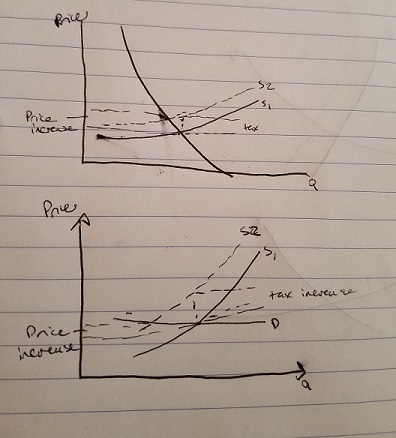
\includegraphics{https://raw.githubusercontent.com/ChristopheHunt/MSDA---Coursework/master/Data\%20609/Homework\%2013/Demand_Curve.jpg}
\caption{}
\end{figure}

\begin{quote}
\end{quote}

\section{Page B-29: problem 1}\label{page-b-29-problem-1}

Consider the graphical model in Figure 15.27. Argue that if the demand
curve fails to shift significantly to the left, an increase in the
equilibrium quantity could occur after the crisis.


\end{document}
